% =====================================================================
%  Основное содержимое отчёта.
% =====================================================================

\labpart{Краткое описание веб-сервера}

\texttt{Caddy} -- веб-сервер общего назначения, отличительная черта
которого -- автоматическое получение и продление TLS-сертификатов
(протокол ACME, по умолчанию Let's Encrypt) без отдельного инструмента
вроде \texttt{certbot}: сертификат запрашивается и обновляется самим
процессом сервера при старте и по мере истечения срока действия. На
сервере \texttt{test-lab4.work.gd} Caddy раздаёт статическую сборку
одностраничного React-приложения (тестовая страница лабораторной
работы), автоматически перенаправляет запросы с HTTP на HTTPS и
записывает каждый запрос в структурированный лог в формате JSON
(\texttt{/var/log/caddy/access.log}) с ротацией по размеру файла.
Конфигурация задаётся декларативным \texttt{Caddyfile} и хранится в
репозитории лабораторной работы (\texttt{Lab4.1-WebServer}) отдельно от
самого сервера, что позволяет пересоздать развёртывание с нуля.

\begin{figure}[H]
  \centering
  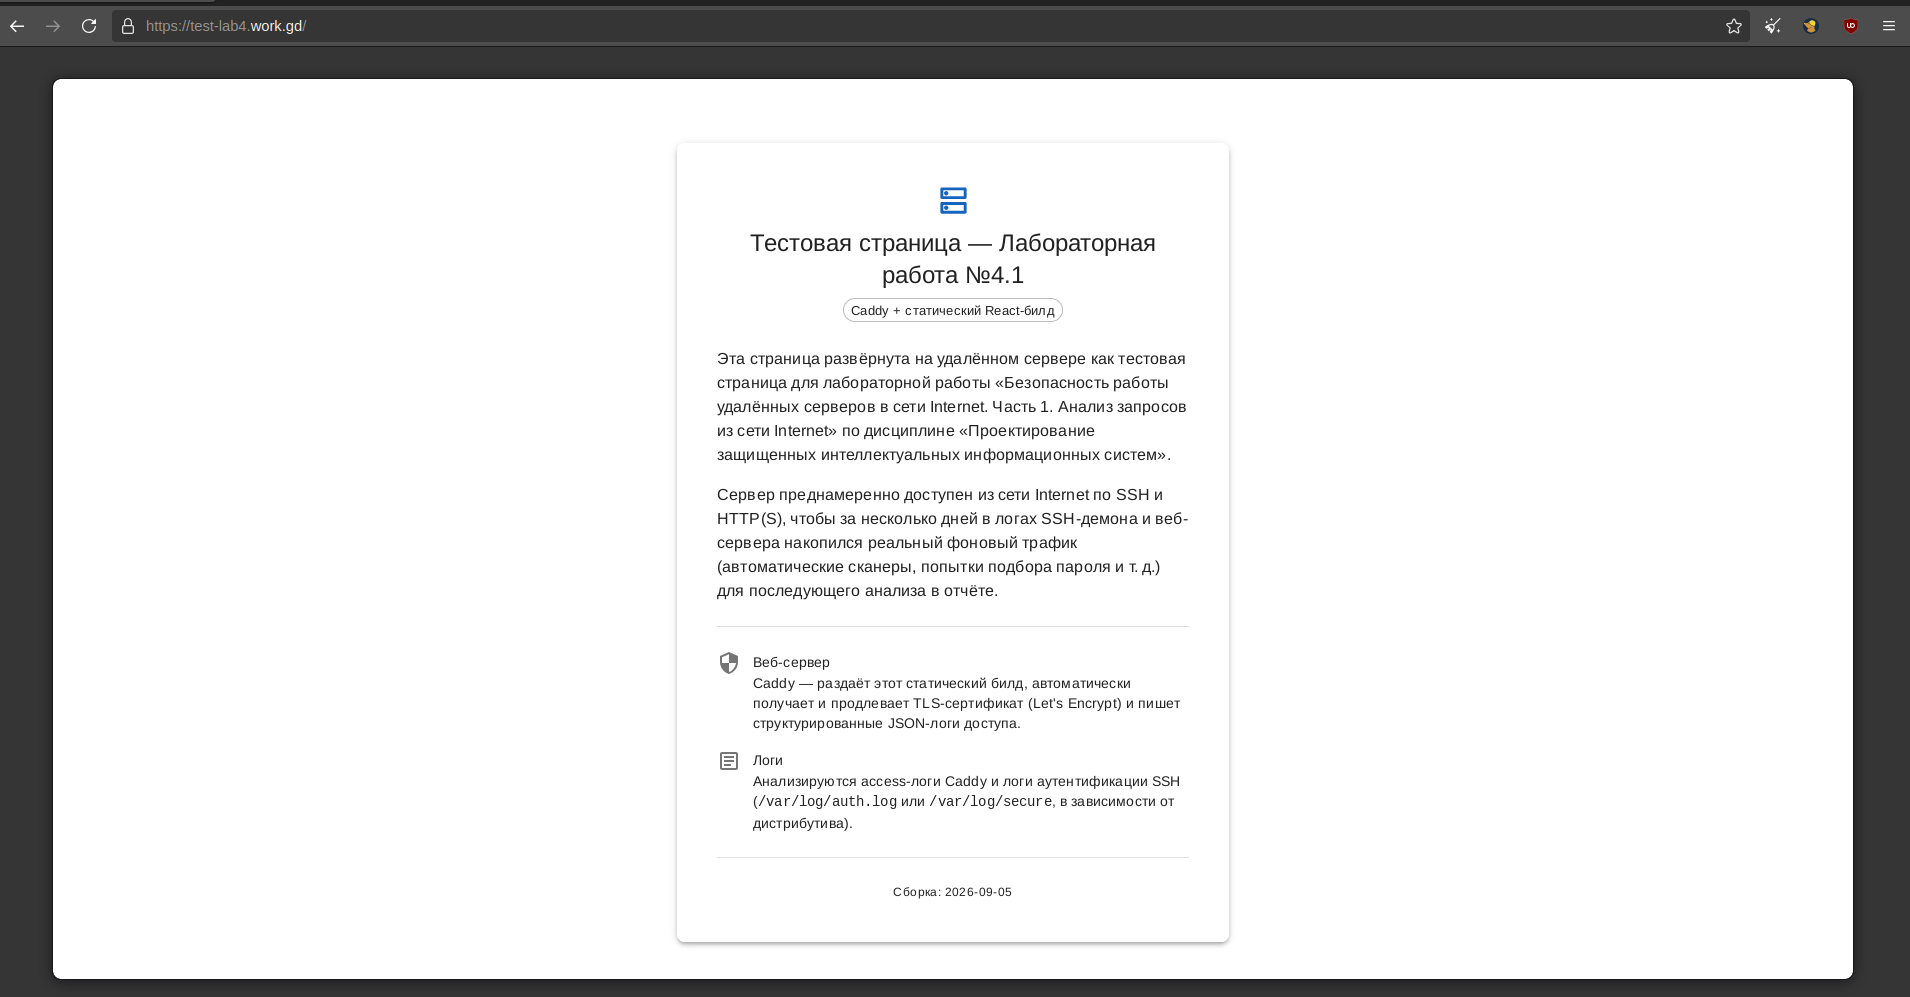
\includegraphics[width=0.8\textwidth]{lab/pictures/testpage-browser.png}
  \caption{Тестовая страница, открытая в браузере по адресу \texttt{https://test-lab4.work.gd/}}
  \label{fig:testpage-browser}
\end{figure}

\labpart{Краткое описание анализируемых файлов}

\begin{itemize}
  \item \textbf{\texttt{/var/log/auth.log}} -- журнал аутентификации
  ОС (Ubuntu/Debian; на CentOS/RHEL аналогичную роль играет
  \texttt{/var/log/secure}), куда демон \texttt{sshd} через
  \texttt{syslog}/\texttt{rsyslog} записывает каждую попытку входа:
  успешную (\texttt{Accepted publickey}/\texttt{password}) и
  неуспешную (\texttt{Failed password}, \texttt{Invalid user}), с
  указанием имени пользователя, IP-адреса источника, времени и способа
  аутентификации. Это основной источник данных для анализа попыток
  подбора учётных данных по SSH.
  \item \textbf{\texttt{/var/log/caddy/access.log}} -- журнал доступа
  веб-сервера, одна строка JSON на каждый HTTP(S)-запрос: IP клиента,
  метод, путь, код ответа, заголовок \texttt{User-Agent}, время
  обработки запроса. Позволяет отличить обращения реальных
  пользователей от автоматических сканеров и ботов по характерным
  путям запроса (например, попытки достучаться до путей вроде
  \texttt{/wp-admin}, административных панелей хостинг-провайдеров и
  т.\,п., которых на самой странице не существует) и по строке
  \texttt{User-Agent}.
\end{itemize}

\labpart{Анализ запросов из сети на SSH сервер и веб-сервер}

\begin{quote}
\textit{Раздел будет заполнен после завершения сбора данных за
несколько дней эксплуатации сервера. Здесь будут приведены: общее
число попыток входа по SSH и их динамика по времени; список наиболее
активных источников (IP-адресов/подсетей) и то, что из этого автоматически
заблокировано системой предотвращения вторжений (см. отчёт по
лабораторной работе №4.2); наиболее часто перебираемые имена
пользователей; статистика запросов к веб-серверу -- объём трафика,
доля обращений к несуществующим путям, характерные \texttt{User-Agent}
сканеров, обнаруженные при первом же запуске сервера (например,
сканер \texttt{LeakIX}).}
\end{quote}

\labpart{Рекомендации по улучшению безопасности удалённого сервера}

\begin{enumerate}
  \item Запретить удалённый вход суперпользователя (\texttt{root})
  через SSH (\texttt{PermitRootLogin no}) и работать через отдельную
  учётную запись с повышением привилегий через \texttt{sudo} -- на
  момент выполнения лабораторной работы \texttt{root} остаётся
  доступен намеренно, чтобы не исказить статистику попыток входа
  именно под этой учётной записью.
  \item Отключить аутентификацию по паролю (\texttt{PasswordAuthentication no}),
  оставив только вход по публичному ключу -- сам подбор пароля тогда
  теряет смысл вне зависимости от его сложности.
  \item Ограничить набор IP-адресов, которым разрешён доступ по SSH
  (например, через \texttt{AllowUsers user@подсеть} или отдельное
  правило firewall), если круг легитимных источников подключения
  заранее известен.
  \item Установить и настроить систему обнаружения/предотвращения
  вторжений (IDS/IPS) для автоматической блокировки источников,
  массово подбирающих пароль или сканирующих сервер -- реализовано и
  подробно разобрано в отчёте по лабораторной работе №4.2.
  \item Свести перечень открытых портов к минимально необходимому
  (22, 80, 443) средствами firewall и логировать заблокированные
  попытки подключения к остальным портам отдельно.
  \item Регулярно анализировать журналы (в идеале -- с автоматическим
  оповещением при превышении порога подозрительной активности), а не
  только пост-фактум, как в рамках этой лабораторной работы.
\end{enumerate}
